\mychapter{Experimental Design}{Experimental Design}{}\label{chap:experimental_design}

\section{Overview}
\label{sec:exp_overview}

This chapter describes how the clarifier classification system was built and configured, and which experiments were run with it. The first part covers the parts of the system that are shared by every experiment: the model architectures and how transfer learning is applied to them (Section~\ref{sec:exp_architectures}), the augmentations applied to the training images (Section~\ref{sec:exp_augmentation}), how the class imbalance in the dataset is handled (Section~\ref{sec:exp_loss}), how the hyperparameters of each architecture were chosen (Section~\ref{sec:exp_hyperparams}), and the training loop itself (Section~\ref{sec:exp_training}).

The second part describes the four experiments that were carried out using this system:

\begin{enumerate}
    \item \textbf{Mixed-facility baseline} (Section~\ref{sec:exp_mixed}): the images of all five facilities are pooled and divided using the stratified 70/20/10 training/validation/test split described in Chapter~\ref{chap:systemmethods}.
    \item \textbf{Leave-one-facility-out evaluation} (Section~\ref{sec:exp_lofo}): each of the five facilities is held out in turn as an unseen test facility, while the model is trained and validated on the remaining four. This is the main experiment of the project, since it estimates how well a model would perform at a facility it has never seen before.
    \item \textbf{Binary (OK / Not-OK) approach} (Section~\ref{sec:exp_binary}): the four clarifier classes are collapsed into a two-class problem, where \textbf{Functional} is treated as OK and \textbf{Dysfunctional}, \textbf{Empty} and \textbf{Scum} are treated as Not-OK.
    \item \textbf{Overview images} (Section~\ref{sec:exp_overview_images}): overview images of the facilities are used instead of the cut out images of individual clarifiers.
\end{enumerate}

The chapter ends with the metrics used to evaluate every run (Section~\ref{sec:exp_metrics}) and the Grad-CAM method used to inspect which parts of an image a model bases its prediction on (Section~\ref{sec:exp_gradcam}).

\begin{figure}[htbp]
\centering
\begin{tikzpicture}[
    node distance=6mm and 12mm,
    stage/.style={rectangle, rounded corners, draw, fill=gray!10, text width=6.8cm, align=center, minimum height=8mm, font=\small},
    arr/.style={-{Stealth[length=2mm]}, thick},
]

\node[stage] (raw) {Raw labelled satellite images (Chapter~\ref{chap:systemmethods})};
\node[stage, below=of raw] (prep) {\texttt{prep.py}: crop labelled regions into per-class image folders (Section~\ref{sec:pipeline})};
\node[stage, below=of prep] (split) {Leave-one-facility-out train / validation / test split (Chapter~\ref{chap:systemmethods})};
\node[stage, below=of split] (aug) {Resize and normalise every image, and randomly augment training images (Section~\ref{sec:exp_augmentation})};
\node[stage, below=of aug] (model) {CNN backbone with a new classifier head (Sections~\ref{sec:exp_architectures} and~\ref{sec:exp_hyperparams})};
\node[stage, below=of model] (train) {Training loop: Adam, \texttt{StepLR}, early stopping (Section~\ref{sec:exp_training})};
\node[stage, below=of train] (results) {Saved per-run results: \texttt{results\_*.pkl} (Section~\ref{sec:exp_lofo})};
\node[stage, below=of results] (compare) {Comparison notebook: cross-architecture, cross-facility results};

\draw[arr] (raw) -- (prep);
\draw[arr] (prep) -- (split);
\draw[arr] (split) -- (aug);
\draw[arr] (aug) -- (model);
\draw[arr] (model) -- (train);
\draw[arr] (train) -- (results);
\draw[arr] (results) -- (compare);

\end{tikzpicture}
\caption{End-to-end experimental pipeline, from labelled satellite imagery to a saved, comparable results file per (architecture, facility) combination.}
\label{fig:experimental_pipeline}
\end{figure}

Figure~\ref{fig:experimental_pipeline} summarises the pipeline from start to finish. It starts from the labelled satellite images described in Chapter~\ref{chap:systemmethods}, which \texttt{prep.py} crops into individual images sorted into one folder per class. These images are then split by facility, so that no image from the held-out test facility is ever used during training. Every image is resized and normalised before it is passed to the network, and images in the training set are also randomly augmented (Section~\ref{sec:exp_augmentation}). The network is one of the seven architectures in Section~\ref{sec:exp_architectures}, with a classifier head sized by the hyperparameters chosen for that architecture (Section~\ref{sec:exp_hyperparams}), and is trained using the loop described in Section~\ref{sec:exp_training}.

The results of every run, meaning one architecture trained with one facility held out, are saved to a separate \texttt{results\_*.pkl} file (Section~\ref{sec:exp_lofo}). Each file contains the test metrics, the confusion matrix, the training history and the prediction made for every test image. Saving the results to disk rather than only keeping them in memory means that the comparison notebook can load the results of every run and compare architectures and facilities in the Results chapter without having to retrain any model.


\section{Model Architectures and Transfer Learning}\label{sec:exp_architectures}

AlexNet is deliberately different from the other six: rather than being fine-tuned from ImageNet weights, it is trained entirely from randomly initialised weights, with its own separate, hand-picked configuration (Section~\ref{sec:exp_hyperparams}). It was added to the project specifically to measure what pretraining itself is worth, that is, whether the far larger pretrained architectures actually outperform a comparatively simple network trained from scratch on this project's own, much smaller dataset, rather than to compete with them on accuracy in its own right.

\begin{table}[htbp]
\centering
\caption{Parameter count of each of the seven architectures evaluated, from smallest to largest.}
\label{tab:arch_sizes}
\begin{tabular}{lc}
\toprule
\textbf{Architecture} & \textbf{Parameters} \\
\midrule
EfficientNet-B0 & 5.3M \\
DenseNet-121    & 8.0M \\
ResNet-18       & 11.7M \\
ResNet-50       & 25.6M \\
Inception-v3    & 27.2M \\
ConvNeXt-Tiny   & 28.6M \\
AlexNet         & 61.1M \\
\bottomrule
\end{tabular}
\end{table}

For each of the six pretrained architectures, transfer learning follows the same recipe. The architecture's convolutional backbone is loaded with weights pretrained on ImageNet~\citep{deng2009imagenet}, specifically torchvision's \texttt{IMAGENET1K\_V1} weights, except for ResNet-50, which uses the newer, more accurate \texttt{IMAGENET1K\_V2} recipe. Its original 1000-class ImageNet output layer is then discarded, and a new classifier head, sized by that architecture's own tuned $H$ and $N$ (Section~\ref{sec:exp_hyperparams}), is put in its place: a stack of $H$ \texttt{Linear+ReLU} pairs followed by a final \texttt{Linear} layer mapping to the project's number of classes. Every parameter in the network, backbone included, is then fine-tuned on the WWTW dataset. No layers are frozen, so pretraining only supplies a starting point for every weight rather than fixing any of them in place.

Exactly which attribute of a given architecture's model object this new head replaces depends on how that architecture happens to be implemented in torchvision, and differs from one architecture to the next: \texttt{model.fc} for ResNet-18, ResNet-50 and Inception-v3, \texttt{model.classifier} for DenseNet-121, and a specific indexed layer within \texttt{model.classifier} for EfficientNet-B0, ConvNeXt-Tiny and AlexNet.

Two architectures need one further, architecture-specific adjustment beyond this. Inception-v3's auxiliary classifier (Section~\ref{sec:inception}), used only during training, also has its own small output layer resized to the project's number of classes; unlike the main classifier head, though, it is always left as a single \texttt{Linear} layer regardless of the tuned $H$ and $N$, since it is only a secondary training signal rather than the model's actual prediction. ConvNeXt-Tiny's global average pooling layer is replaced with global max pooling, so the feature vector reaching its classifier head is built from each channel's strongest activation rather than its average.


\section{Augmentation}
\label{sec:exp_augmentation}

Data augmentation makes small, random changes to the training images, so that the network sees a slightly different version of every image each time it is used. This increases the variety in the training data without collecting any new images, and makes it harder for the network to memorise individual images. Augmentation is applied to the training set only. The validation and test images are never augmented, so that they are evaluated exactly as they are.

The augmentations are applied on the fly by PyTorch each time an image is loaded, rather than being generated once and saved to disk. The size of the training set therefore stays the same, but every epoch sees a new, randomly augmented version of each training image. Three augmentations are applied, in the following order:

\begin{itemize}
    \item \textbf{Horizontal flip}: the image is mirrored from left to right with a probability of 50\%.
    \item \textbf{Rotation}: the image is rotated by a random angle, chosen uniformly between $-15^\circ$ and $+15^\circ$. The output image keeps its original size, so the corners that are rotated out of the frame are cut off, and the empty corners that are rotated into the frame are filled with black.
    \item \textbf{Colour jitter}: the brightness, contrast, saturation and hue of the image are changed by a random amount, with the four adjustments applied in a random order. The brightness and contrast are each multiplied by a random factor between $0.6$ and $1.4$, the saturation by a random factor between $0.7$ and $1.3$, and the hue is shifted by up to $\pm 0.1$ of the full colour wheel (at most $36^\circ$).
\end{itemize}

The flip and rotation are suited to this dataset because the images are taken from directly above. A clarifier seen from above has no fixed orientation, so a mirrored or slightly rotated clarifier is still a realistic example of the same class. Since the clarifier crops are already masked to black outside the circular tank (Section~\ref{sec:pipeline}), the black corners introduced by the rotation also blend in with the existing background.

The colour jitter targets a different problem. The images come from different facilities and were captured on different dates, so the lighting, sun glare and water colour vary between images. The colour jitter is intended to stop the network from memorising the exact colour or brightness of the water at a particular facility, and to make it rely on other features of the clarifier instead.

The hue shift does raise a concern, since the clarifier classes are partly defined by colour, and a \textbf{Dysfunctional} clarifier is identified by its green surface (Chapter~\ref{chap:systemmethods}). A hue shift could wash out this green colour while the image keeps its \textbf{Dysfunctional} label. To test whether this harmed the models, all seven architectures were retrained on all five leave-one-facility-out splits with the hue shift disabled, keeping every other augmentation and hyperparameter the same. This did not improve performance. The mean test accuracy decreased for every architecture, by between 0.1 and 3.1 percentage points for the six pretrained architectures, and the number of correctly identified \textbf{Dysfunctional} clarifiers did not improve consistently. The hue shift was therefore kept.

Figure~\ref{fig:augmentation_examples} shows these augmentations applied to a single training image. The top row shows each augmentation on its own, while the bottom row shows four random outputs of the full augmentation pipeline, as the network would see them during training.

\begin{figure}[htbp]
    \centering
    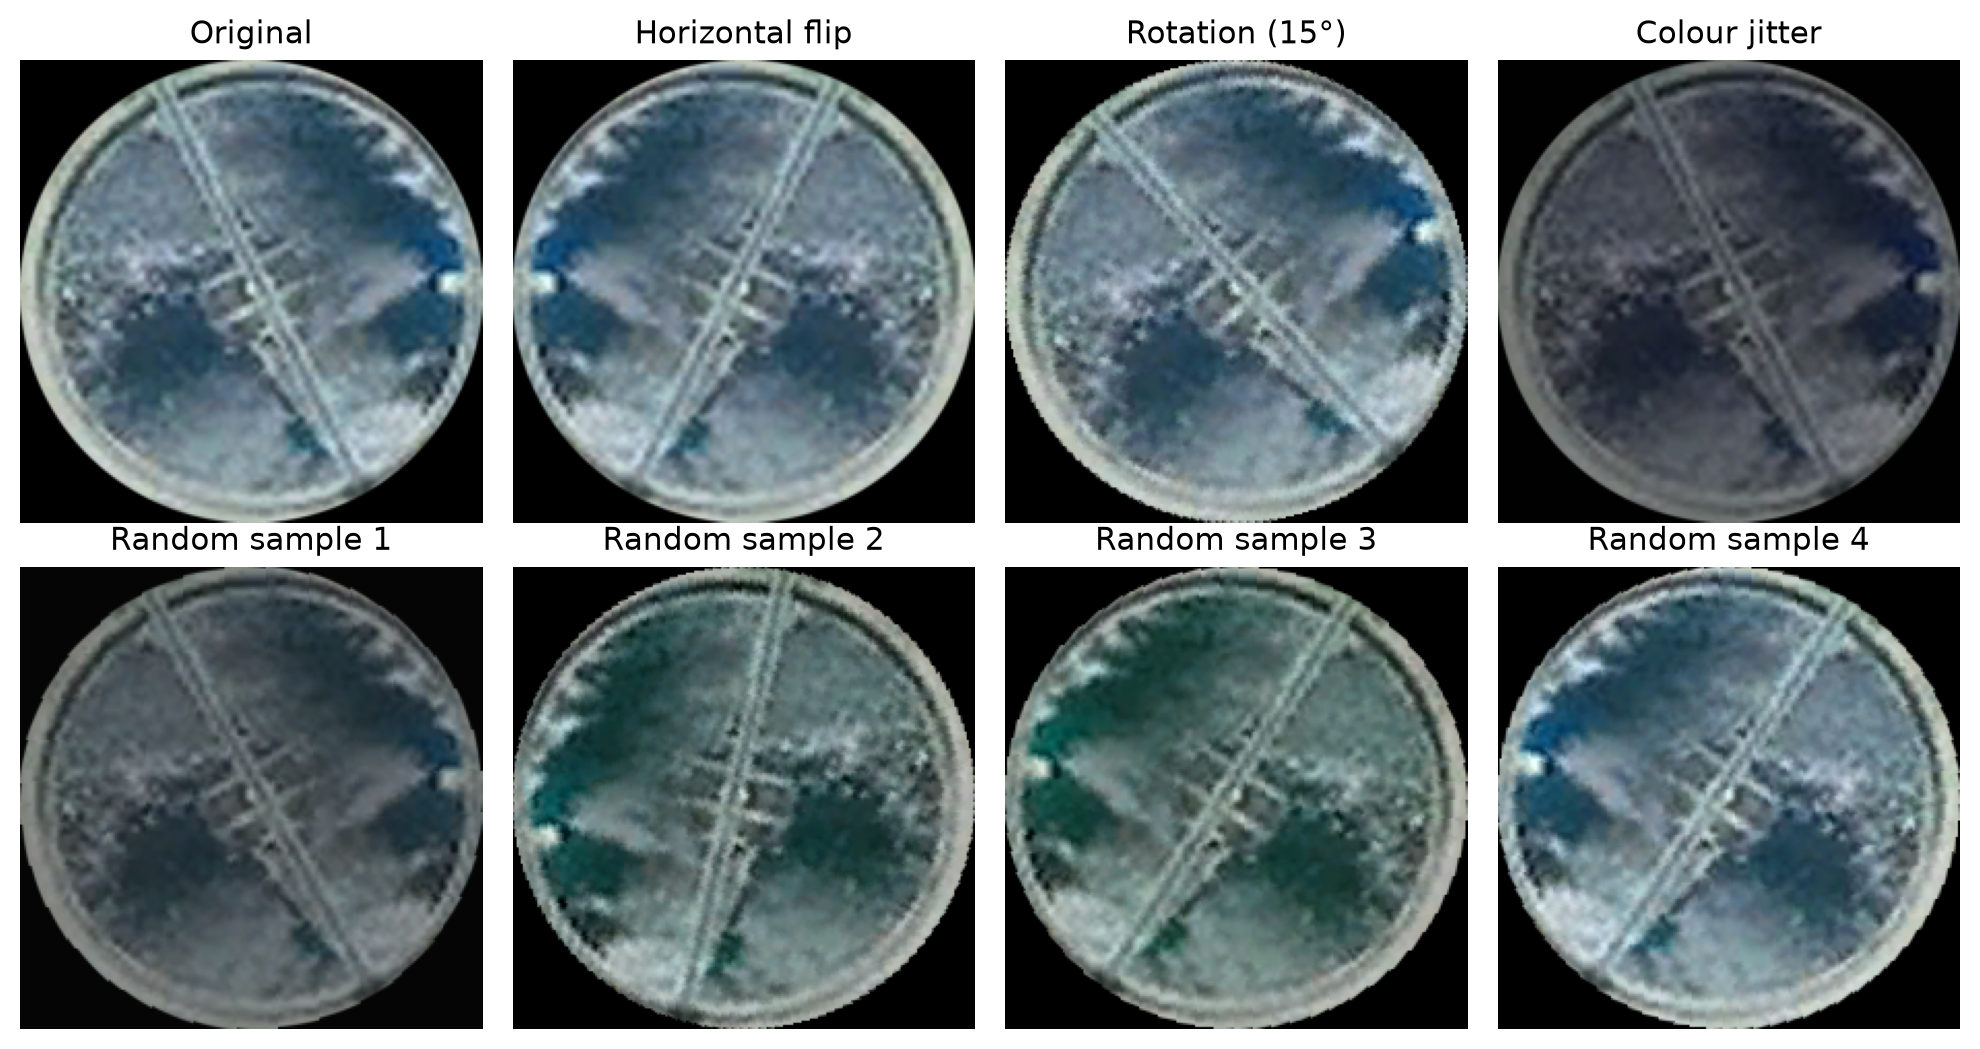
\includegraphics[width=0.9\textwidth]{figures/augmentation_examples.png}
    \caption{Augmentations applied to a single \textbf{Scum} clarifier from Cape Flats. Top row: the original image, followed by a horizontal flip, a rotation of $15^\circ$, and a random colour jitter, each applied on its own. Bottom row: four random outputs of the full augmentation pipeline (flip, rotation and colour jitter combined).}
    \label{fig:augmentation_examples}
\end{figure}


\section{Class Imbalance}
\label{sec:exp_loss}

As shown in Table~\ref{tab:clarifier_summary}, the clarifier classes are far from balanced. \textbf{Functional} and \textbf{Scum} clarifiers make up most of the dataset, while \textbf{Dysfunctional} and especially \textbf{Empty} clarifiers are much less common. If every image contributes equally to the loss, the network can reach a low loss by mostly predicting the common classes, and has little incentive to learn the rare ones.

To counter this, the cross-entropy loss is weighted per class, so that the network is penalised more for misclassifying an image from a rare class than from a common one. The weight of each class is inversely proportional to the number of training images in that class, and the weights are then normalised so that they sum to the number of classes. For $K$ classes, where $n_c$ is the number of training images in class $c$, the weight of class $c$ is

\begin{equation}
    w_c = K \cdot \frac{1/n_c}{\sum_{j=1}^{K} 1/n_j}.
\end{equation}

A class with average representation therefore gets a weight close to one, a rare class gets a weight larger than one, and a common class gets a weight smaller than one. These weights are passed to PyTorch's \texttt{CrossEntropyLoss}, which multiplies the loss of each image by the weight of its true class. The training data itself is not resampled, so every training image is still used exactly once per epoch.

The weights are calculated from the training set only, and are recalculated for every leave-one-facility-out split. This is necessary because the class counts change depending on which facility is held out. Table~\ref{tab:class_weights} lists the training images per class and the resulting weights for each of the five splits.

\begin{table}[htbp]
\centering
\caption{Number of training images per clarifier class and the resulting class weight $w_c$, for each held-out test facility.}
\label{tab:class_weights}
\begin{tabular}{l cc cc cc cc}
\toprule
& \multicolumn{2}{c}{\textbf{Dysfunctional}} & \multicolumn{2}{c}{\textbf{Empty}} & \multicolumn{2}{c}{\textbf{Functional}} & \multicolumn{2}{c}{\textbf{Scum}} \\
\cmidrule(lr){2-3} \cmidrule(lr){4-5} \cmidrule(lr){6-7} \cmidrule(lr){8-9}
\textbf{Test facility} & \scriptsize{Images} & \scriptsize{$w_c$} & \scriptsize{Images} & \scriptsize{$w_c$} & \scriptsize{Images} & \scriptsize{$w_c$} & \scriptsize{Images} & \scriptsize{$w_c$} \\
\midrule
Atlantis       & 221 & 1.48 & 196 & 1.67 & 750 & 0.44 & 778 & 0.42 \\
Cape Flats     & 133 & 0.56 & 25  & 2.97 & 253 & 0.29 & 417 & 0.18 \\
Fisantekraal   & 206 & 1.50 & 190 & 1.63 & 690 & 0.45 & 728 & 0.42 \\
Northern Works & 109 & 2.10 & 183 & 1.25 & 714 & 0.32 & 686 & 0.33 \\
Waterval       & 215 & 1.48 & 198 & 1.60 & 705 & 0.45 & 671 & 0.47 \\
\bottomrule
\end{tabular}
\end{table}

The Cape Flats split stands out. Cape Flats contains 214 of the 245 \textbf{Empty} clarifiers in the dataset (Table~\ref{tab:relabel_corrections}), so when it is held out for testing, only 25 \textbf{Empty} images are left for training. The weight of the \textbf{Empty} class rises to 2.97 as a result, more than sixteen times the weight of the \textbf{Scum} class (0.18). In the same way, Northern Works contains 140 of the 273 \textbf{Dysfunctional} clarifiers, so holding it out raises the \textbf{Dysfunctional} weight to 2.10.

The same weighted loss is also used to calculate the validation loss. Since the validation loss decides when training stops early and which epoch's weights are kept (Section~\ref{sec:exp_training}), the class weighting also influences model selection, and not only the gradient updates during training.


\section{Hyperparameter Tuning}
\label{sec:exp_hyperparams}

Some of the parameters were fixed, and are the same for every architecture. These values were never changed, either because a well-established default already exists or because there was no reason to expect the best value to depend on the architecture. This covers Adam's $\beta_2$ term (kept at $0.999$, the default recommended in Adam's original paper and rarely changed in practice), the $L_2$ weight decay ($10^{-4}$, a standard mild regularisation strength), and the training loop's own settings: a maximum of 100 epochs, an early-stopping patience of 10 epochs, and a fixed random seed of 42.

Every other hyperparameter, namely the classifier head's shape (hidden layers $H$ and neurons per layer $N$), the learning rate, Adam's $\beta_1$, the \texttt{StepLR} step size, and the batch size, was tuned automatically using Optuna~\cite{akiba2019optuna}, a hyperparameter optimisation library, for six of the project's seven architectures: ResNet-18, ResNet-50, DenseNet-121, Inception-v3, EfficientNet-B0, and ConvNeXt-Tiny. AlexNet is excluded, since it is trained from scratch rather than fine-tuned from ImageNet weights, and is instead given a fixed, hand-picked configuration (Section~\ref{subsec:defaults}).

\subsection{Why Optuna}
\label{subsec:why_optuna}

These six hyperparameters interact with each other, so tuning them one at a time risks a setting that is only good in combination with values chosen later. A grid search over all six jointly is not practical either, since the number of combinations grows multiplicatively and each training run already takes several minutes to over an hour. Optuna instead searches all six jointly using a Tree-structured Parzen Estimator (TPE) sampler, which uses the trials seen so far to sample new candidates from the regions of the search space that have scored well, rather than sampling blindly. Alongside it, a \texttt{MedianPruner} monitors each trial's validation accuracy after every epoch and stops a trial early once it falls behind the median of the other trials at that same epoch, so a clearly uncompetitive trial does not run to completion. Together these let a fixed budget of 20 trials per architecture cover the search space far more efficiently than 20 random guesses would.

Tuning all six architectures under all five leave-one-facility-out splits would multiply an already substantial compute cost by five, so tuning was instead carried out once per architecture, on a single held-out-facility split (Northern Works held out for testing), and the winning combination is applied uniformly across all five folds when the architecture is actually trained (Section~\ref{sec:exp_lofo}).

Table~\ref{tab:search_space} lists the search space explored for every architecture.

\begin{table}[htbp]
\centering
\caption{The hyperparameter search space explored by Optuna, shared by all six tuned architectures. Learning rate is sampled log-uniformly, so values across the full range are equally likely on a log scale.}
\label{tab:search_space}
\begin{tabular}{lll}
\toprule
\textbf{Hyperparameter} & \textbf{Symbol} & \textbf{Candidate values / range} \\
\midrule
Hidden layers            & $H$        & $\{0, 1, 2, 3\}$ \\
Neurons per layer        & $N$        & $\{512, 1024, 2048\}$ \\
Batch size                & --         & $\{8, 16, 24, 32, 48, 64, 96, 128\}$ \\
Learning rate              & --         & $[10^{-6}, 10^{-2}]$ (log-uniform) \\
Adam $\beta_1$              & $\beta_1$  & $[0.5, 0.999]$ \\
\texttt{StepLR} step size    & --         & $[5, 40]$ (integer) \\
\bottomrule
\end{tabular}
\end{table}

A classifier head with $H{=}0$ hidden layers is a single linear layer mapping straight from the backbone's features to the class scores, with $N$ unused; Optuna selected this for EfficientNet-B0 (Section~\ref{subsec:tune_effnetb0}).

The six subsections below give, for each tuned architecture, the search range and winning value for every hyperparameter. A trial either \emph{completes} (reporting a final validation accuracy) or is \emph{pruned}: stopped early either by the \texttt{MedianPruner} for underperforming, or, for a small number of trials on EfficientNet-B0 and ConvNeXt-Tiny, by an intermittent GPU driver fault that killed the training process outright and unrelated to the hyperparameters being tested. Every architecture's tuning run started from the same fixed sampler seed, which is why Trial~0 samples the same combination in every table. All 20 trials for every architecture are listed in Appendix~\ref{appen:hyperparam_trials}.

\subsection{ResNet-18}
\label{subsec:tune_resnet18}

Of ResNet-18's 20 trials, 14 completed and 6 were pruned. Table~\ref{tab:tuned_resnet18} gives the search range and the winning value for each hyperparameter; all 20 trials are listed in Table~\ref{tab:trials_resnet18}, Appendix~\ref{appen:hyperparam_trials}.

\begin{table}[htbp]
\centering
\caption{ResNet-18: search range and the value ultimately chosen for each tuned hyperparameter, from the winning trial (\#11, validation accuracy 89.27\%).}
\label{tab:tuned_resnet18}
\begin{tabular}{lll}
\toprule
\textbf{Hyperparameter} & \textbf{Search range} & \textbf{Chosen value} \\
\midrule
Hidden layers ($H$)      & $\{0, 1, 2, 3\}$                  & 2 \\
Neurons per layer ($N$)  & $\{512, 1024, 2048\}$              & 2048 \\
Learning rate             & $[10^{-6}, 10^{-2}]$ (log-uniform) & $3.88\times10^{-4}$ \\
Adam $\beta_1$            & $[0.5, 0.999]$                     & 0.611 \\
StepLR step size           & $[5, 40]$ (integer)                & 12 \\
Batch size                 & $\{8,16,24,32,48,64,96,128\}$      & 96 \\
\bottomrule
\end{tabular}
\end{table}

\subsection{EfficientNet-B0}
\label{subsec:tune_effnetb0}

Of EfficientNet-B0's 20 trials, 10 completed and 10 were pruned, including 3 that were cut short by the GPU driver fault mentioned above rather than the pruner itself. Table~\ref{tab:tuned_effnetb0} gives the search range and the winning value for each hyperparameter; all 20 trials are listed in Table~\ref{tab:trials_effnetb0}, Appendix~\ref{appen:hyperparam_trials}.

\begin{table}[htbp]
\centering
\caption{EfficientNet-B0: search range and the value ultimately chosen for each tuned hyperparameter, from the winning trial (\#16, validation accuracy 88.54\%).}
\label{tab:tuned_effnetb0}
\begin{tabular}{lll}
\toprule
\textbf{Hyperparameter} & \textbf{Search range} & \textbf{Chosen value} \\
\midrule
Hidden layers ($H$)      & $\{0, 1, 2, 3\}$                  & 0 \\
Neurons per layer ($N$)  & $\{512, 1024, 2048\}$              & -- (unused) \\
Learning rate             & $[10^{-6}, 10^{-2}]$ (log-uniform) & $4.89\times10^{-4}$ \\
Adam $\beta_1$            & $[0.5, 0.999]$                     & 0.857 \\
StepLR step size           & $[5, 40]$ (integer)                & 5 \\
Batch size                 & $\{8,16,24,32,48,64,96,128\}$      & 96 \\
\bottomrule
\end{tabular}
\end{table}

\subsection{DenseNet-121}
\label{subsec:tune_densenet121}

Of DenseNet-121's 20 trials, 16 completed and 4 were pruned. Table~\ref{tab:tuned_densenet121} gives the search range and the winning value for each hyperparameter; all 20 trials are listed in Table~\ref{tab:trials_densenet121}, Appendix~\ref{appen:hyperparam_trials}.

\begin{table}[htbp]
\centering
\caption{DenseNet-121: search range and the value ultimately chosen for each tuned hyperparameter, from the winning trial (\#19, validation accuracy 90.24\%).}
\label{tab:tuned_densenet121}
\begin{tabular}{lll}
\toprule
\textbf{Hyperparameter} & \textbf{Search range} & \textbf{Chosen value} \\
\midrule
Hidden layers ($H$)      & $\{0, 1, 2, 3\}$                  & 1 \\
Neurons per layer ($N$)  & $\{512, 1024, 2048\}$              & 512 \\
Learning rate             & $[10^{-6}, 10^{-2}]$ (log-uniform) & $3.44\times10^{-4}$ \\
Adam $\beta_1$            & $[0.5, 0.999]$                     & 0.597 \\
StepLR step size           & $[5, 40]$ (integer)                & 11 \\
Batch size                 & $\{8,16,24,32,48,64,96,128\}$      & 48 \\
\bottomrule
\end{tabular}
\end{table}

\subsection{ResNet-50}
\label{subsec:tune_resnet50}

Of ResNet-50's 20 trials, 15 completed and 5 were pruned. Table~\ref{tab:tuned_resnet50} gives the search range and the winning value for each hyperparameter; all 20 trials are listed in Table~\ref{tab:trials_resnet50}, Appendix~\ref{appen:hyperparam_trials}.

\begin{table}[htbp]
\centering
\caption{ResNet-50: search range and the value ultimately chosen for each tuned hyperparameter, from the winning trial (\#11, validation accuracy 89.02\%).}
\label{tab:tuned_resnet50}
\begin{tabular}{lll}
\toprule
\textbf{Hyperparameter} & \textbf{Search range} & \textbf{Chosen value} \\
\midrule
Hidden layers ($H$)      & $\{0, 1, 2, 3\}$                  & 2 \\
Neurons per layer ($N$)  & $\{512, 1024, 2048\}$              & 2048 \\
Learning rate             & $[10^{-6}, 10^{-2}]$ (log-uniform) & $3.77\times10^{-4}$ \\
Adam $\beta_1$            & $[0.5, 0.999]$                     & 0.875 \\
StepLR step size           & $[5, 40]$ (integer)                & 17 \\
Batch size                 & $\{8,16,24,32,48,64,96,128\}$      & 96 \\
\bottomrule
\end{tabular}
\end{table}

\subsection{ConvNeXt-Tiny}
\label{subsec:tune_convnext}

Of ConvNeXt-Tiny's 20 trials, 13 completed and 7 were pruned, including 1 that was cut short by the GPU driver fault mentioned above rather than the pruner itself. Table~\ref{tab:tuned_convnext} gives the search range and the winning value for each hyperparameter; all 20 trials are listed in Table~\ref{tab:trials_convnext}, Appendix~\ref{appen:hyperparam_trials}.

\begin{table}[htbp]
\centering
\caption{ConvNeXt-Tiny: search range and the value ultimately chosen for each tuned hyperparameter, from the winning trial (\#17, validation accuracy 90.73\%).}
\label{tab:tuned_convnext}
\begin{tabular}{lll}
\toprule
\textbf{Hyperparameter} & \textbf{Search range} & \textbf{Chosen value} \\
\midrule
Hidden layers ($H$)      & $\{0, 1, 2, 3\}$                  & 1 \\
Neurons per layer ($N$)  & $\{512, 1024, 2048\}$              & 2048 \\
Learning rate             & $[10^{-6}, 10^{-2}]$ (log-uniform) & $5.65\times10^{-5}$ \\
Adam $\beta_1$            & $[0.5, 0.999]$                     & 0.560 \\
StepLR step size           & $[5, 40]$ (integer)                & 21 \\
Batch size                 & $\{8,16,24,32,48,64,96,128\}$      & 128 \\
\bottomrule
\end{tabular}
\end{table}

\subsection{Inception-v3}
\label{subsec:tune_inceptionv3}

Of Inception-v3's 20 trials, 13 completed and 7 were pruned. Table~\ref{tab:tuned_inceptionv3} gives the search range and the winning value for each hyperparameter; all 20 trials are listed in Table~\ref{tab:trials_inceptionv3}, Appendix~\ref{appen:hyperparam_trials}.

\begin{table}[htbp]
\centering
\caption{Inception-v3: search range and the value ultimately chosen for each tuned hyperparameter, from the winning trial (\#1, validation accuracy 89.51\%).}
\label{tab:tuned_inceptionv3}
\begin{tabular}{lll}
\toprule
\textbf{Hyperparameter} & \textbf{Search range} & \textbf{Chosen value} \\
\midrule
Hidden layers ($H$)      & $\{0, 1, 2, 3\}$                  & 2 \\
Neurons per layer ($N$)  & $\{512, 1024, 2048\}$              & 2048 \\
Learning rate             & $[10^{-6}, 10^{-2}]$ (log-uniform) & $1.38\times10^{-3}$ \\
Adam $\beta_1$            & $[0.5, 0.999]$                     & 0.600 \\
StepLR step size           & $[5, 40]$ (integer)                & 23 \\
Batch size                 & $\{8,16,24,32,48,64,96,128\}$      & 96 \\
\bottomrule
\end{tabular}
\end{table}

\subsection{Summary Across Architectures}
\label{subsec:tune_summary}

Table~\ref{tab:full_hyperparams} draws the winning configuration for each of the six tuned architectures together into a single reference table, alongside the hand-picked configuration used for AlexNet.

\begin{table}[htbp]
\centering
\footnotesize
\caption{Final training configuration used for every architecture: the winning Optuna trial for the six tuned architectures (Table~\ref{tab:tuned_resnet18} through Table~\ref{tab:tuned_inceptionv3}), and the hand-picked values used for AlexNet (Section~\ref{subsec:defaults}).}
\label{tab:full_hyperparams}
\begin{tabular}{lcccccc}
\toprule
\textbf{Architecture} & \textbf{$H$} & \textbf{$N$} & \textbf{LR} & \textbf{$\beta_1$} & \textbf{Step size} & \textbf{Batch size} \\
\midrule
ResNet-18 (tuned)       & 2 & 2048 & $3.88\times10^{-4}$ & 0.611 & 12 & 96  \\
ResNet-50 (tuned)       & 2 & 2048 & $3.77\times10^{-4}$ & 0.875 & 17 & 96  \\
DenseNet-121 (tuned)    & 1 & 512  & $3.44\times10^{-4}$ & 0.597 & 11 & 48  \\
Inception-v3 (tuned)    & 2 & 2048 & $1.38\times10^{-3}$ & 0.600 & 23 & 96  \\
EfficientNet-B0 (tuned) & 0 & --   & $4.89\times10^{-4}$ & 0.857 & 5  & 96  \\
ConvNeXt-Tiny (tuned)   & 1 & 2048 & $5.65\times10^{-5}$ & 0.560 & 21 & 128 \\
AlexNet (hand-picked)   & 3 & 1024 & $1\times10^{-3}$    & 0.9   & 15 & 32  \\
\bottomrule
\end{tabular}
\end{table}

A pattern worth noting across the six searches: every one of them settled on a $\beta_1$ below the conventional Adam default of $0.9$, ranging from $0.560$ (ConvNeXt-Tiny) to $0.875$ (ResNet-50). This suggests that, for fine-tuning these particular pretrained backbones on this dataset, slightly less momentum (i.e.\ weighting each step more towards the current batch's gradient and less towards the accumulated direction of previous steps) consistently outperformed the textbook default, even though the search was free to select values as high as $0.999$.

\subsection{AlexNet's Hand-Picked Configuration}
\label{subsec:defaults}

AlexNet (Table~\ref{tab:full_hyperparams}) was never passed through the Optuna search at all: as noted at the start of this section, it is trained entirely from randomly initialised weights rather than fine-tuned from an ImageNet-pretrained backbone (Section~\ref{sec:exp_architectures}), so a search tuned around fine-tuning behaviour is not guaranteed to transfer to it. Its configuration was instead chosen by hand, with each value reasoned through individually rather than picked arbitrarily:

\begin{itemize}
    \item \textbf{$H{=}3$, $N{=}1024$}: a reasonably deep, moderately wide head, deep enough to give the classifier some capacity to work with, without adding the largest possible number of parameters ($N{=}2048$) to a head sitting on top of a backbone that, unlike the other six architectures, has not already learned any useful features.
    \item \textbf{Learning rate $=10^{-3}$}: an order of magnitude higher than a typical fine-tuning learning rate. This is a deliberate departure, not an oversight: with no pretrained features to preserve, a learning rate suited to gently fine-tuning an already-good set of weights would instead be needlessly slow at moving a randomly initialised network away from its starting point, so a higher learning rate suited to training from scratch was used instead.
    \item \textbf{$\beta_1{=}0.9$}: Adam's own textbook default, for the same reason $\beta_2$ is fixed at its own default throughout this project (Section~\ref{sec:exp_hyperparams}): a well-established default value with no particular reason to expect it to be wrong.
    \item \textbf{Step size $=15$}: with \texttt{StepLR} cutting the learning rate by a factor of ten every 15 epochs against a maximum of 100, this decays the learning rate roughly a third of the way into a full run, which is a reasonable middle point given the tuned step sizes found by the search for the other six architectures ranged from as early as epoch 5 (EfficientNet-B0) to as late as epoch 23 (Inception-v3).
    \item \textbf{Batch size $=32$}: a conventional default batch size for image classification, small enough to need no gradient accumulation beyond what \texttt{MICRO\_BATCH\_CAP} already imposes on every architecture.
\end{itemize}


\section{Training Procedure}
\label{sec:exp_training}

Every architecture is trained with the same underlying loop; only the specific hyperparameter values (learning rate, batch size, and so on) change per architecture, as set out in Section~\ref{sec:exp_hyperparams}. This section covers that loop itself: how the learning rate changes over a run, when training stops, and which weights are actually kept.

Rather than using one fixed learning rate for an entire run, every architecture uses \texttt{StepLR} to cut the learning rate by a factor of ten after a fixed, architecture-specific number of epochs (Section~\ref{sec:exp_hyperparams}), since large steps are useful early on to make fast progress but become counter-productive once the model is close to a good solution, where they cause it to overshoot instead of settling in.

Training is allowed to run for up to 100 epochs, but is stopped early if validation loss has not improved for 10 consecutive epochs, since the point at which a given architecture stops improving and starts overfitting is not known ahead of time and differs from one architecture to the next. Validation \emph{loss}, rather than accuracy, is used to decide both when to stop and which epoch's weights to keep: whichever epoch achieved the lowest validation loss is the one whose weights are restored and carried forward to testing, rather than simply whatever weights training happened to end on. Figure~\ref{fig:training_flow} summarises this loop.

\begin{figure}[htbp]
\centering
\begin{tikzpicture}[
    node distance=7mm and 12mm,
    process/.style={rectangle, rounded corners, draw, fill=gray!10, text width=4.3cm, align=center, minimum height=8mm, font=\small},
    decision/.style={diamond, draw, fill=blue!5, aspect=2.2, text width=3.4cm, align=center, inner sep=1pt, font=\small},
    terminal/.style={rectangle, rounded corners=3mm, draw, fill=gray!25, text width=3.4cm, align=center, minimum height=7mm, font=\small},
    arr/.style={-{Stealth[length=2mm]}, thick},
    lbl/.style={font=\scriptsize}
]

\node[terminal] (start) {Start (epoch 1)};
\node[process, below=of start] (trainval) {Train one epoch, then evaluate on the validation set};
\node[process, below=of trainval] (lrstep) {Step the \texttt{StepLR} schedule};
\node[decision, below=of lrstep] (improved) {Validation loss improved?};
\node[process, below left=9mm and -8mm of improved] (savebest) {Save weights as new best checkpoint; reset counter to 0};
\node[process, below right=9mm and -8mm of improved] (noimprove) {Increment no-improvement counter};
\node[decision, below=18mm of improved] (stopcheck) {Counter $\geq$ 10, or epoch 100 reached?};
\node[terminal, below=of stopcheck] (restore) {Restore best checkpoint};
\node[terminal, below=of restore] (end) {Proceed to testing};

\draw[arr] (start) -- (trainval);
\draw[arr] (trainval) -- (lrstep);
\draw[arr] (lrstep) -- (improved);
\draw[arr] (improved.west) -| node[lbl, pos=0.25, above]{Yes} (savebest.north);
\draw[arr] (improved.east) -| node[lbl, pos=0.25, above]{No} (noimprove.north);
\draw[arr] (savebest.south) |- (stopcheck.west);
\draw[arr] (noimprove.south) |- (stopcheck.east);
\draw[arr] (stopcheck) -- node[lbl, right]{Yes} (restore);
\draw[arr] (restore) -- (end);

\draw[arr] (stopcheck.west) -| ++(-3.2,0) |- node[lbl, pos=0.05, above, sloped]{No, next epoch} (trainval.west);

\end{tikzpicture}
\caption{The training loop used for every architecture: an epoch of training and validation, a scheduler step, a checkpoint decision based on validation loss, and a stopping check repeated every epoch until training ends.}
\label{fig:training_flow}
\end{figure}

Inception-v3 is trained with one additional detail: during training only, it produces a second, auxiliary prediction partway through the network, and the loss from this auxiliary output is added to the main loss at a reduced weight of $0.4$. This gives the earlier layers of the network a more direct training signal than would otherwise reach them through such a deep network, and is discarded entirely once training finishes, playing no role in the model's actual predictions at test time.

The same fixed seed used throughout this project (Section~\ref{sec:exp_hyperparams}) also covers the random initialisation of each architecture's new classifier head, in addition to the dataset shuffling and splitting described in Chapter~\ref{chap:systemmethods}, so that a given experiment can be reproduced exactly if re-run.


\section{Experiment 1: Mixed-Facility Baseline}
\label{sec:exp_mixed}

% \begin{itemize}
%     \item Describe this as the project's first/original experimental setup: all five facilities pooled, then split with the stratified 70/20/10 train/val/test split already described in Chapter~\ref{chap:systemmethods}.
%     \item State which architectures were evaluated under this setup (the four originally available: ResNet-18 baseline, ResNet-50, DenseNet-121, Inception-v3) and that this is also the setup under which the hyperparameter tuning in Section~\ref{sec:exp_hyperparams} was performed.
%     \item Explain the purpose of this experiment: establish a best-case, "easy" performance figure where training and test images are drawn from the same facilities (and therefore similar lighting, camera, water colour, etc.), before testing something harder.
%     \item Explain \emph{why} this setup is insufficient on its own, motivating Experiment 2: a stratified split can leak facility-specific "shortcut" cues into both train and test (e.g.\ a particular facility's water always looking a certain colour), so high accuracy here does not guarantee the model would work at a facility it has never seen — which is the actual deployment scenario described in Chapter~\ref{chap:introduction}.
% \end{itemize}

TODO


\section{Experiment 2: Leave-One-Facility-Out Evaluation}
\label{sec:exp_lofo}

% \begin{itemize}
%     \item Cross-reference Chapter~\ref{chap:systemmethods}, Section~\ref{sec:pipeline} for exactly how each leave-one-out split is constructed (Figure~\ref{fig:leave_one_out approach}); this section covers how that split is used experimentally.
%     \item Describe the full experimental grid run via \texttt{run.py}: all 6 architectures $\times$ all 5 facilities (Atlantis, Cape Flats, Waterval, Fisantekraal, Northern Works) held out in turn = 30 (architecture, held-out facility) training runs per component, run unattended as a batch (via \texttt{jupyter nbconvert --execute}) so a full sweep doesn't need to be babysat.
%     \item Explain that this is the main/current experiment the project's results are based on, and why: it measures accuracy on a facility whose images never influenced training \emph{or} model selection in any way, which is the realistic test of whether the system would work at a genuinely new facility.
%     \item Describe what gets saved per run (\texttt{results\_\allowbreak<component>\_\allowbreak<architecture>\_\allowbreak<facility>.pkl}): test accuracy, mean AUC, full classification report (precision/recall/F1 per class), confusion matrix, training history, and a per-sample record of every test image's path/true label/predicted label — explain why this is saved (so later analysis, e.g.\ qualitative error inspection or Grad-CAM, doesn't need the GPU or the trained model again).
%     \item Mention the comparison notebook (\texttt{results\_comparison.ipynb}) briefly here as \emph{how} results are assembled across the grid, saving the actual comparison for the Results chapter: it loads every available results file, builds a facility $\times$ architecture comparison table, and produces grouped bar charts of test accuracy/mean AUC by held-out facility.
% \end{itemize}

TODO


\section{Experiment 3: Binary (OK / Not-OK) Reformulation}
\label{sec:exp_binary}

TODO


\section{Experiment 4: Overview Images}
\label{sec:exp_overview_images}
TODO


\section{Evaluation Metrics}
\label{sec:exp_metrics}

\begin{itemize}
    \item List and justify each metric collected per run:
    \begin{itemize}
        \item \textbf{Accuracy}
        \item \textbf{Per-class precision/recall/F1} and the \textbf{confusion matrix}
        \item \textbf{Loss graphs}
        \item \textbf{AUC}
    \end{itemize}
    \item Explain why recall is an important metric in this project's context.
\end{itemize}


\section{Qualitative Analysis: Grad-CAM}
\label{sec:exp_gradcam}

\begin{itemize}
    \item State the purpose.
    \item Describe the method.
    \item show example Grad-CAM visualisations for both a correct and an incorrect prediction, and discuss what they reveal about the model's behaviour.
\end{itemize}

\begin{figure}[htbp]
    \centering
    \fbox{\parbox{0.7\textwidth}{\centering\vspace{3cm} PLACEHOLDER: example image alongside its Grad-CAM heatmap overlay, for both a correct and an incorrect prediction \vspace{3cm}}}
    \caption{PLACEHOLDER: Grad-CAM visualisation showing which image regions the model attends to when making a prediction.}
    \label{fig:gradcam_example}
\end{figure}


